\section[Approach]{Our Approach to the Problem}
\label{sys:appr}
We took a black-box approach to find out the prevalence of this vulnerability on the World Wide Web. According to \cite{wiki:Black-box_testing}:
\begin{quote}
	``{Black-box testing is a method of software testing that examines the functionality of an application without peering into its internal structures or workings.}''
\end{quote} 

Since we did not have the source code for each of these websites (and even if we did, the sheer number of websites would have made it a \emph{very} tall task), black-box testing was the ideal approach for this project.
Black-box testing gave us the freedom to not worry about the underlying code for the website under test, letting us concentrate on the payload instead. A high level logical overview of our system is presented in Figure~\ref{fig:overall}.

\begin{figure}
	\centering
	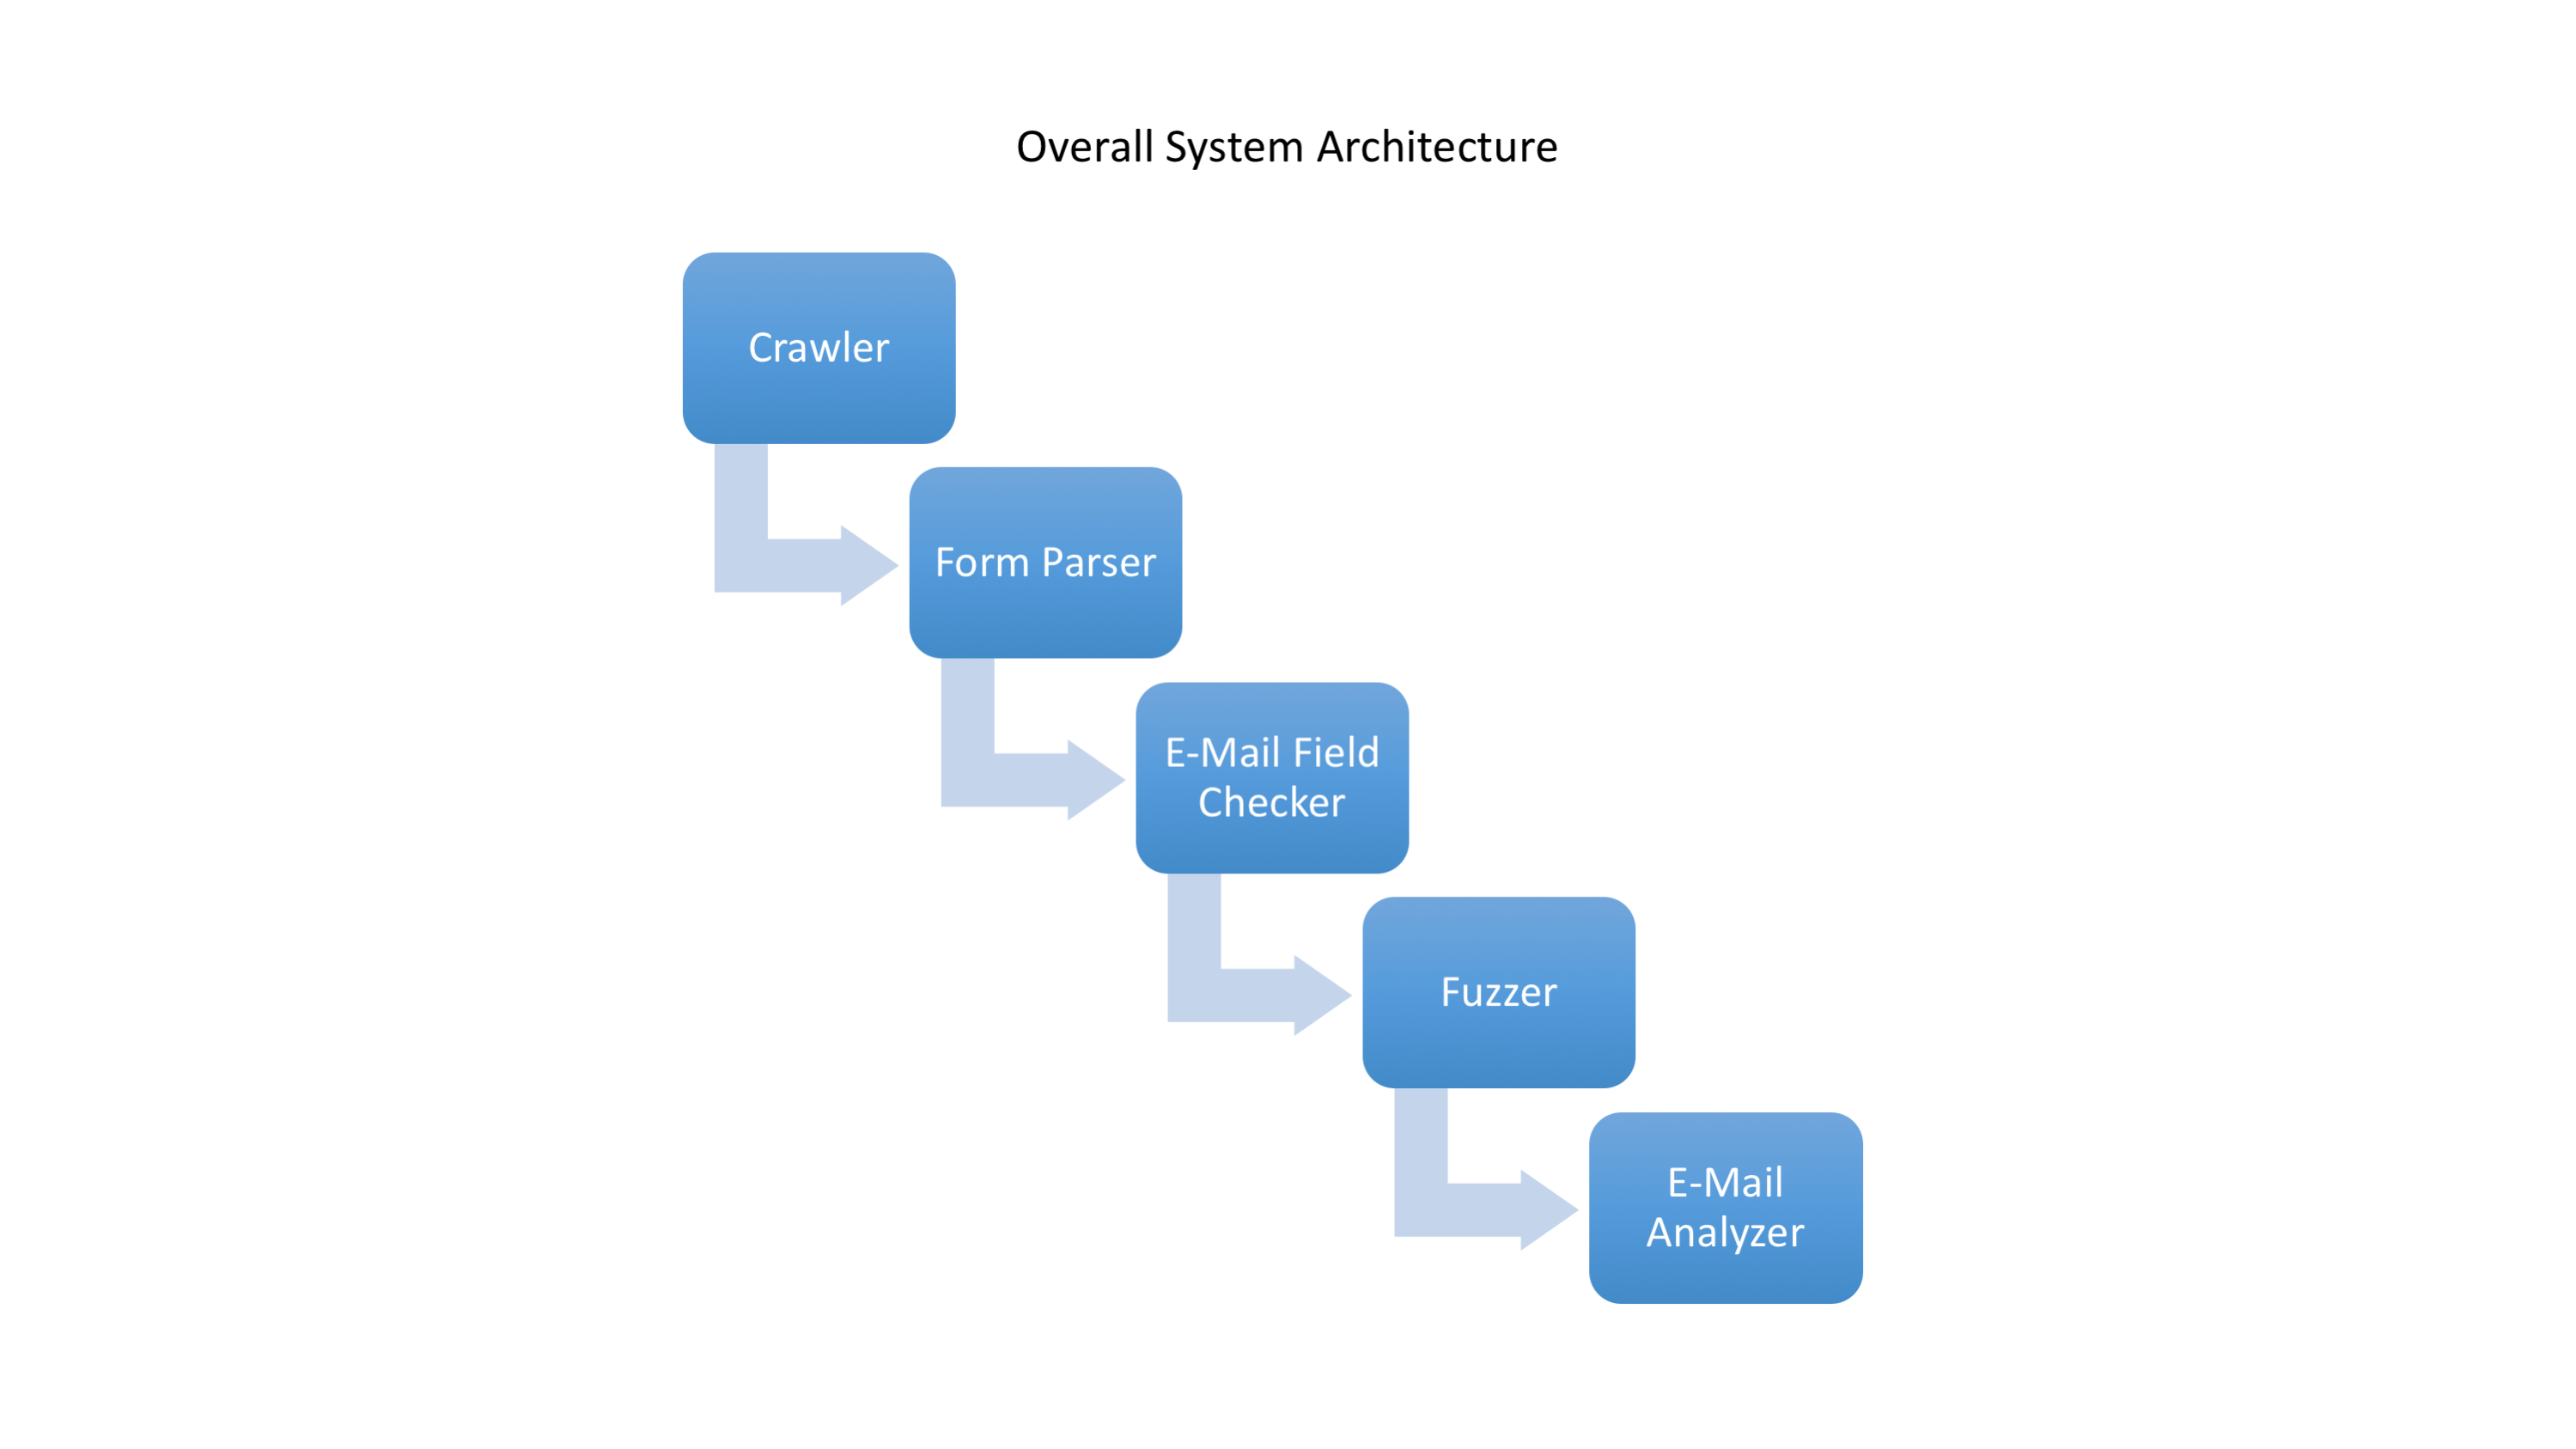
\includegraphics[width=14cm, height=7cm]{System/overall_design}
	\caption[\titlecap{Overall system architecture - logical overview}]{Overall system architecture - logical overview.}
	\label{fig:overall}
\end{figure}
